\subsection{Memory Layout in Computer Systems}

In modern computer systems, memory is divided into several distinct segments that each serve a different purpose in the execution of a program. These segments include the stack, heap, and various regions that hold code and data. This section provides a mathematical description of the layout of memory in a typical system and explains the role of each memory segment.

\subsubsection{Memory Segments}

A typical program is divided into the following memory segments:

\begin{table}[h]
	\centering
	\begin{tabular}{|c|l|}
		\hline
		\multirow{2}{*}{\textbf{Stack}} & Used for local variables, function call management, and control flow. \\
		& It grows downward in memory. \\ \hline
		\multirow{2}{*}{\textbf{Heap}} & Used for dynamic memory allocation (e.g., via \texttt{malloc}). \\ & It grows upward in memory. \\ \hline
		\textbf{.text} & Stores the program's executable instructions (machine code). \\ \hline
		\textbf{.data} & Stores initialized global and static variables. \\ \hline
		\multirow{2}{*}{\textbf{.bss}} & Stores uninitialized global and static variables. \\
		& This segment is initialized to zero at runtime. \\ \hline
		\textbf{.rodata} & Stores read-only data, such as string literals or constant variables. \\ \hline
	\end{tabular}
	%	\caption{Summary of memory segments in a typical program.}
\end{table}
\begin{itemize}
	\item \textbf{Stack:} Used for local variables, function call management, and control flow. It grows downward in memory.
	\item \textbf{Heap:} Used for dynamic memory allocation (e.g., via \texttt{malloc}). It grows upward in memory.
	\item \textbf{.text:} Stores the program's executable instructions (machine code).
	\item \textbf{.data:} Stores initialized global and static variables.
	\item \textbf{.bss:} Stores uninitialized global and static variables. This segment is initialized to zero at runtime.
	\item \textbf{.rodata:} Stores read-only data, such as string literals or constant variables.
\end{itemize}

\noindent The memory layout in a typical process can be visualized as:

\begin{center}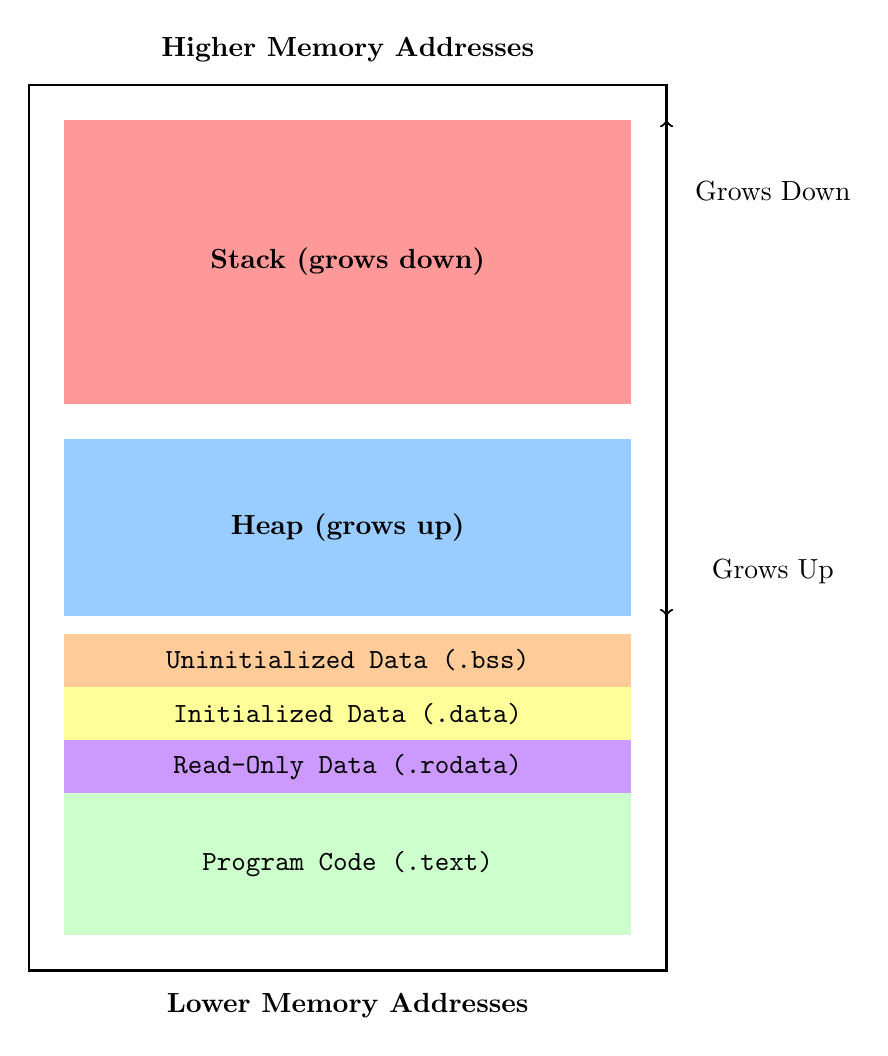
\begin{tikzpicture}[scale=.9]
		% Define colors for segments
		\definecolor{stackcolor}{RGB}{255, 153, 153}
		\definecolor{heapcolor}{RGB}{153, 204, 255}
		\definecolor{textcolor}{RGB}{204, 255, 204}
		\definecolor{datacolor}{RGB}{255, 255, 153}
		\definecolor{bsscolor}{RGB}{255, 204, 153}
		\definecolor{rodatacolor}{RGB}{204, 153, 255}
		
		% Base address
		\node at (0,10.5) {\textbf{Higher Memory Addresses}};
		\node at (0,-3.0) {\textbf{Lower Memory Addresses}};
		
		% Expanded width for rectangles (from -4 to 4)
		% Stack
		\fill[stackcolor] (-4, 5.5) rectangle (4, 9.5);
		\node at (0,7.5) {\textbf{Stack (grows down)}};
		
		% Heap
		\fill[heapcolor] (-4, 2.5) rectangle (4, 5);
		\node at (0,3.75) {\textbf{Heap (grows up)}};
		
		% BSS
		\fill[bsscolor] (-4, 1.5) rectangle (4, 2.25);
		\node at (0,1.875) {\texttt{Uninitialized Data (.bss) }};
		
		% Data
		\fill[datacolor] (-4, 0.75) rectangle (4, 1.5);
		\node at (0,1.125) {\texttt{Initialized Data (.data)}};
		
		% ROData
		\fill[rodatacolor] (-4, 0) rectangle (4, 0.75);
		\node at (0,0.375) {\texttt{Read-Only Data (.rodata)}};
		
		% Text
		\fill[textcolor] (-4, -2) rectangle (4, 0);
		\node at (0,-1) {\texttt{Program Code (.text)}};
		
		% Annotations and arrows
		\draw[thick,->] (4.5,7.5) -- (4.5,9.5);
		\node at (6,8.5) {Grows Down};
		
		\draw[thick,->] (4.5,3.75) -- (4.5,2.5);
		\node at (6,3.125) {Grows Up};
		
		% Memory boundary lines (Expand to match rectangle width)
		\draw[thick] (-4.5, -2.5) rectangle (4.5, 10);
\end{tikzpicture}\end{center}